% --------------------------------------
% Document Class
% --------------------------------------
\documentclass[a4paper,11pt]{article}
% --------------------------------------



% --------------------------------------
% Use Package
% --------------------------------------


\usepackage[francais]{babel}
%\usepackage{ucs}
\usepackage[utf8]{inputenc}
\usepackage[T1]{fontenc}

\usepackage{makeidx}
\usepackage{color}
\usepackage{graphicx}
\usepackage{float}
\usepackage[hidelinks]{hyperref} 
\usepackage{geometry}
%\usepackage{lastpage}
%\usepackage{marginnote}
\usepackage{fancyhdr}
%\usepackage{titlesec}
%\usepackage{framed}
\usepackage{amsmath}
\usepackage{empheq}
\usepackage{array}
\usepackage{multicol}
\usepackage{csquotes}
%\usepackage{adjustbox}

% insert code
\usepackage{listings}

% define our color
\usepackage{xcolor}

% code color
\definecolor{ligthyellow}{RGB}{250,247,220}
\definecolor{darkblue}{RGB}{5,10,85}
\definecolor{ligthblue}{RGB}{1,147,128}
\definecolor{darkgreen}{RGB}{8,120,51}
\definecolor{darkred}{RGB}{160,0,0}

% other color
\definecolor{ivi}{RGB}{141,107,185}


\lstset{
    language=Scilab,
    captionpos=b,
    extendedchars=true,
    frame=lines,
    numbers=left,
    numberstyle=\tiny,
    numbersep=5pt,
    keepspaces=true,
    breaklines=true,
    showspaces=false,
    showstringspaces=false,
    breakatwhitespace=false,
    stepnumber=1,
    showtabs=false,
    tabsize=3,
    basicstyle=\small\ttfamily,
    backgroundcolor=\color{ligthyellow},
    keywordstyle=\color{ligthblue},
    morekeywords={include, printf, uchar},
    identifierstyle=\color{darkblue},
    commentstyle=\color{darkgreen},
    stringstyle=\color{darkred},
}


% --------------------------------------



% --------------------------------------
% Page setting
% --------------------------------------
%\pagestyle{empty}
\setlength{\headheight}{15pt}

\setcounter{secnumdepth}{3}
\setcounter{tocdepth}{2}

\makeatletter
\@addtoreset{chapter}{part}
\makeatother 

\hypersetup{         % parametrage des hyperliens
  colorlinks=true,      % colorise les liens
  breaklinks=true,      % permet les retours à la ligne pour les liens trop longs
  urlcolor= blue,       % couleur des hyperliens
  linkcolor= black,     % couleur des liens internes aux documents (index, figures, tableaux, equations,...)
  citecolor= green      % couleur des liens vers les references bibliographiques
}

% --------------------------------------

% --------------------------------------
% Information
% --------------------------------------
\title{Compte-rendu TP9 TI : Détection de contours par approches du premier ordre}
\author{Elliot VANEGUE et Gaëtan DEFLANDRE}
% --------------------------------------

\definecolor{myColor}{rgb}{0.5, 0.1, 0.75}

% --------------------------------------
% Begin content
% --------------------------------------
\begin{document}

% Set language to english
  \selectlanguage{francais}

  % Start the page counting
  \pagenumbering{arabic}

  \maketitle
  
  \mbox{}
  \newpage
  \clearpage
  
  \section*{Introduction}
  Lors de ce TP, nous allons chercher à déterminer les contours d'une image grâce aux 
  gradients de ses pixels. Ces gradients porte de nombreuse information qui peuvent
  être déterminé grâce à l'algorithme de Sobel, qui calcul le vecteur des gradients.
  
  \section{Seuillage de la norme d'un gradient}
  
  Nous avons dans un premier temps calculé les dérivées partielle de la fonction image dans 
  les directions horizontal et vertical. Pour cela, nous appliquons les filtres de Sobel
  $\begin{pmatrix}
     -1 & 0 & 1 \\
     -2 & 0 & 2 \\
     -1 & 0 & 1 
  \end{pmatrix}$ et 
   $\begin{pmatrix}
     -1 & -2 & -1 \\
     0 & 0 & 0 \\
     1 & 2 & 1
  \end{pmatrix}$
  Afin de calculer le gradient de chaque pixel dans la direction x et y.
  Nous obtenons ainsi une image avec les contours dont la direction est horizontal et une seconde avec les contours vertical.\\
  
  \begin{figure}[H]
  \center
   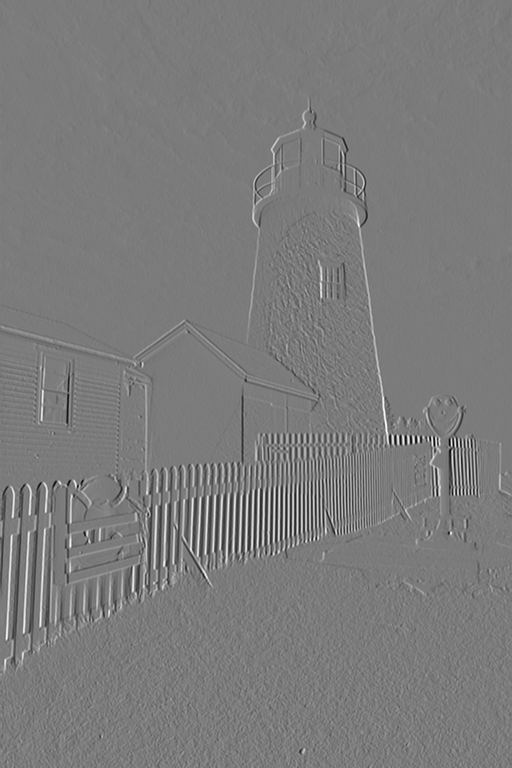
\includegraphics[width=5cm]{../lighthouse_8bits_grad_x.png}
   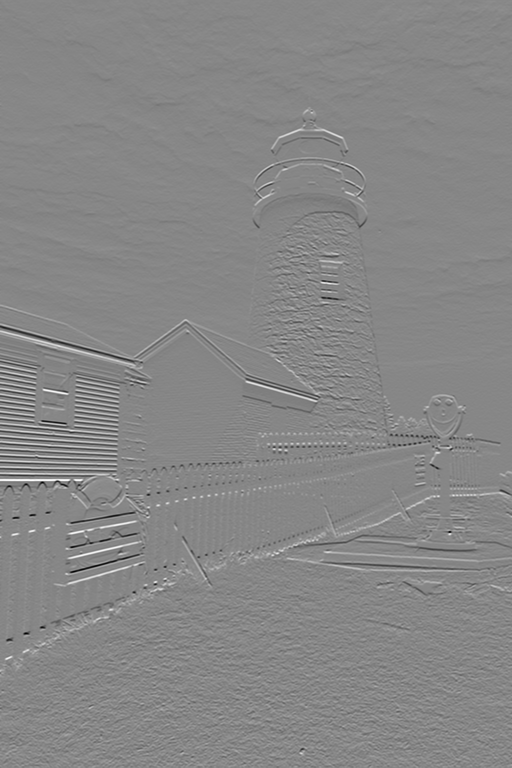
\includegraphics[width=5cm]{../lighthouse_8bits_grad_y.png}
   \caption{Images avec les contours horizontal et vertical}
  \end{figure}

  On voit sur ces deux images que les contours détecté par chaque filtre ne sont pas les mêmes
  à cause de leur direction. Grâce au valeur des pixels de ces deux images, nous calculons la norme
  des gradiants dans une nouvelle image, ce qui fera ressortir des contours de l'image.

  \begin{figure}[H]
  \center
   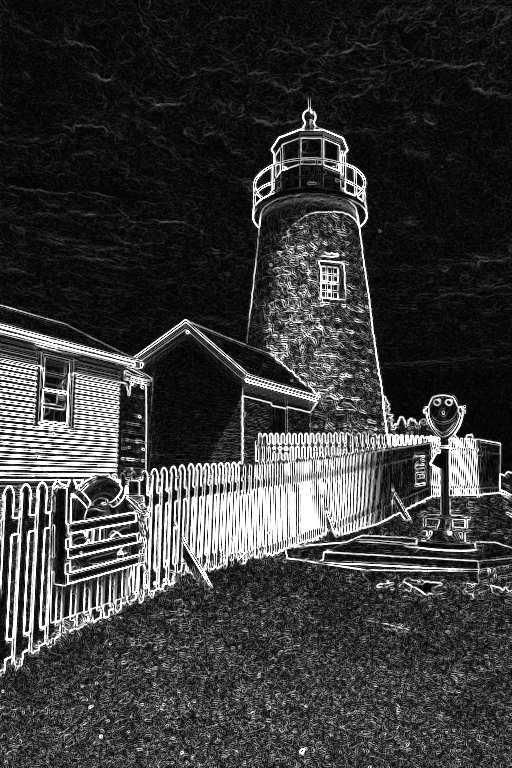
\includegraphics[width=5cm]{../norme8.png}
   \caption{Norme de l'image}
  \end{figure}
  
  On voit que la norme fait bien ressortir les contours, mais certain d'entre eux sont incomplet
  ou à l'inverse trop épais. Quand on regarde l'histogramme de l'image on voit que le minimum est 0
  et le maximum est 904.
  
\end{document}  